\documentclass[10pt]{article}

% PACKAGES ---------------------------------------------------------------
\usepackage{fullpage}
\usepackage{amsmath}
\usepackage{amsfonts}
\usepackage{amsthm}
\usepackage{bm}
\usepackage{graphicx}
\usepackage{amssymb}
\usepackage[usenames]{color}
\usepackage{url}

% DEFINITIONS ------------------------------------------------------------
\newcommand{\CMPLX}{\ensuremath{\mathbb{C}}}
\newcommand{\REAL}{\ensuremath{\mathbb{R}}}
\newcommand{\supp}{\ensuremath{\mbox{\textrm{supp }}}}
\providecommand{\abs}[1]{\lvert#1\rvert} \providecommand{\norm}[1]{\lVert#1\rVert}
\newcommand{\comment}[1]{} % makes its argument disappear

\theoremstyle{plain}
\newtheorem{thm}{Theorem}[section]
\newtheorem{cor}[thm]{Corollary}
\newtheorem{lem}[thm]{Lemma}
\newtheorem{prop}[thm]{Proposition}
\theoremstyle{definition}
\newtheorem{defn}{Definition}[section]
\newtheorem{rem}[thm]{Remark}
\newtheorem{example}{\textsc{Example}}[section]
%\numberwithin{table}{section} \numberwithin{equation}{section} \numberwithin{figure}{section}

\definecolor{MyDarkBlue}{rgb}{0.1,0,0.95}
\newcommand{\MLP}[1]{\textcolor{MyDarkBlue}{[#1]}}
\definecolor{MyOrange}{rgb}{.87,.45,.09}
\newcommand{\DJL}[1]{\textcolor{MyOrange}{[#1]}}

%%% ----------------------------------------------------------------------
\title{Software Requirement Specifications \\for Multi-Physics Peridynamics Simulation Code}
\author{Michael L. Parks, David J. Littlewood, Stewart A. Silling, John A. Mitchell}

\begin{document}

%%% ----------------------------------------------------------------------
\maketitle
%%% ----------------------------------------------------------------------

%%% ----------------------------------------------------------------------
%\renewcommand{\thefootnote}{\fnsymbol{footnote}}
%\footnotetext[2]{mlparks@sandia.gov}
%\footnotetext[3]{djlittl@sandia.gov}
%\footnotetext[4]{sasilli@sandia.gov}
%\renewcommand{\thefootnote}{\arabic{footnote}}
%%% ----------------------------------------------------------------------

%%% ----------------------------------------------------------------------
\section{Introduction} \label{sec:Introduction}

\subsection{Purpose}

This document states the requirements of a rapid production massively parallel multiphysics simulation code based upon peridynamics. These requirements stated serve as an acceptance procedure for this software system. This document contains design elements and is also intended as a starting point for a preliminary implementation.

\subsection{Scope}

This software system will provide a multiphysics simulation capability for peridynamic models. The working name for the code is \emph{\textbf{Peridigm}}.

\paragraph{What \emph{Peridigm} is:}

The software product will perform multiphysics peridynamics simulations, be optimization-enabled, have born-in uncertainty quantification (UQ), exhibit good scalability, be usable as a stand-alone code, will contain modules suitable for incorporation into Sierra Mechanics where appropriate, and will allow for the potential integration of existing material models (e.g.~the Lam\'{e} material library).

It will run in both in a serial (single processor) mode and in a parallel mode, using MPI. The implementation will allow for easy modification and extension with new functionality.

It will be open-source under a suitable public license. As per current 1400 policy, the goal is not to generate revenue through product sales, but instead to capture \emph{mindshare} and recognition as \emph{thought leaders} through development and innovation.

This software will be be maintained by the developers and new features will be added, pending continued funding, as driven by customer demands.

\paragraph{What \emph{Peridigm} is not:}

This software system does not employ a graphical user interface, nor does it provide means for plotting or visualization of data. It does not automagically provide constitutive models for arbitrary materials or physics, nor a means to automagically couple arbitrary physics. It does not perform complex mesh/grid generation but will mesh simple geometric solids, including rectangular solids and cylindrical solids.

\paragraph{Objectives.} This software system will constitute the first open source production quality massively parallel multiphysics peridynamics code, using the state-based formulation of peridynamics \cite{Silling:2007:PDStates}.

\paragraph{Benefit.} This software system will provide a unified mathematical and computational framework for multiphysics simulations.

\paragraph{Goals.} This software system will realize an instantiation of the plan and approach being developed in Andy Salinger's \emph{Agile Components} work (e.g., demonstrate the approach and process of rapidly developing a production-quality application code from pre-existing components). In addition to illustrating how components can be assembled into a production code, the infrastructure needed to rapidly prototype a wider variety of simulation codes will be further established by producing any needed additional components.

\subsection{Definitions, acronyms, and abbreviations}

\begin{description}
  \item[BLAS:] Basic Linear Algebra Subroutines
  \item[Boost:] The Boost C++ libraries are a collection of peer-reviewed, open source libraries that extend the functionality of C++.
  \item[CMake:] Cross-Platform Make, a cross-platform, open-source make system. CMake is used to control the software compilation process using simple platform and compiler independent configuration files.
  \item[CTest:] CTest is a testing tool distributed as a part of CMake, and is used to automate testing.
  \item[DAKOTA:] The DAKOTA (Design Analysis Kit for Optimization and Terascale Applications) toolkit \cite{Eldred:2008:Dakota} provides a flexible, extensible interface between analysis codes and iteration methods.
  \item[PD:] Peridynamics \cite{Silling:2000:PD,Silling:2005:Meshfree,Silling:2007:PDStates}.
  \item[LAPACK:] Linear Algebra PACKage
  \item[MPL:] Metaprogramming library.
  \item[SRS:] Software Requirement Specifications.
  \item[Subversion:] Open-source revision control system.
  \item[TPL:] Third Party Library
  \item[Trac:] Project management and bug/issue tracking system with interface to Subversion and integrated wiki.
  \item[Trilinos:] The Trilinos Project \cite{Heroux:2005:Trilinos} is an effort to develop algorithms and enabling technologies within an object-oriented software framework for the solution of large-scale, complex multi-physics engineering and scientific problems.
  \item[UQ:] Uncertainty quantification.
  \item[VOTD:] Version Of The Day.
\end{description}

\subsection{References}
\bibliographystyle{siam}
\bibliography{PDDesignDocument}

\subsection{Overview}

\noindent
Section \ref{sec:Description} provides an overview of the software's purpose and intended functionality.  Included in Section~\ref{sec:Description} are a description of general user characteristics and the code's relationship to external libraries.  Section~\ref{sec:Requirements} consists of detailed requirements descriptions for hardware and software interfaces, functionality and performance, development tools, and software testing. The appendix contains an outline for the order that features should be implemented.

%%% ----------------------------------------------------------------------
\section{Overall Description} \label{sec:Description}

\subsection{Product perspective}

This project is intended to realize an instantiation of the ongoing \emph{Agile Components} work and also to provide the first open source production quality massively parallel multiphysics peridynamics code. As it matures, this code is intended to support multiphysics and also multiscale peridynamic simulations at Sandia and in the larger academic and industrial community.

The software deliverable will function as a stand-alone analysis code and will contain modules suitable for integration into Sierra Mechanics and/or other analysis codes where appropriate.  Examples of functionality that will be modularized for incorporation into other analysis codes include:
\begin{itemize}
\item The calculation of peridynamic deformation states;
\item The calculation of peridynamic force states;
\item An interface allowing for the adaptation of classical material models for use in peridynamic analyses;
\item Data structures for storing peridynamics-specific information (e.g., neighbor list).
\end{itemize}

\begin{figure}[h!]
  \begin{center}
   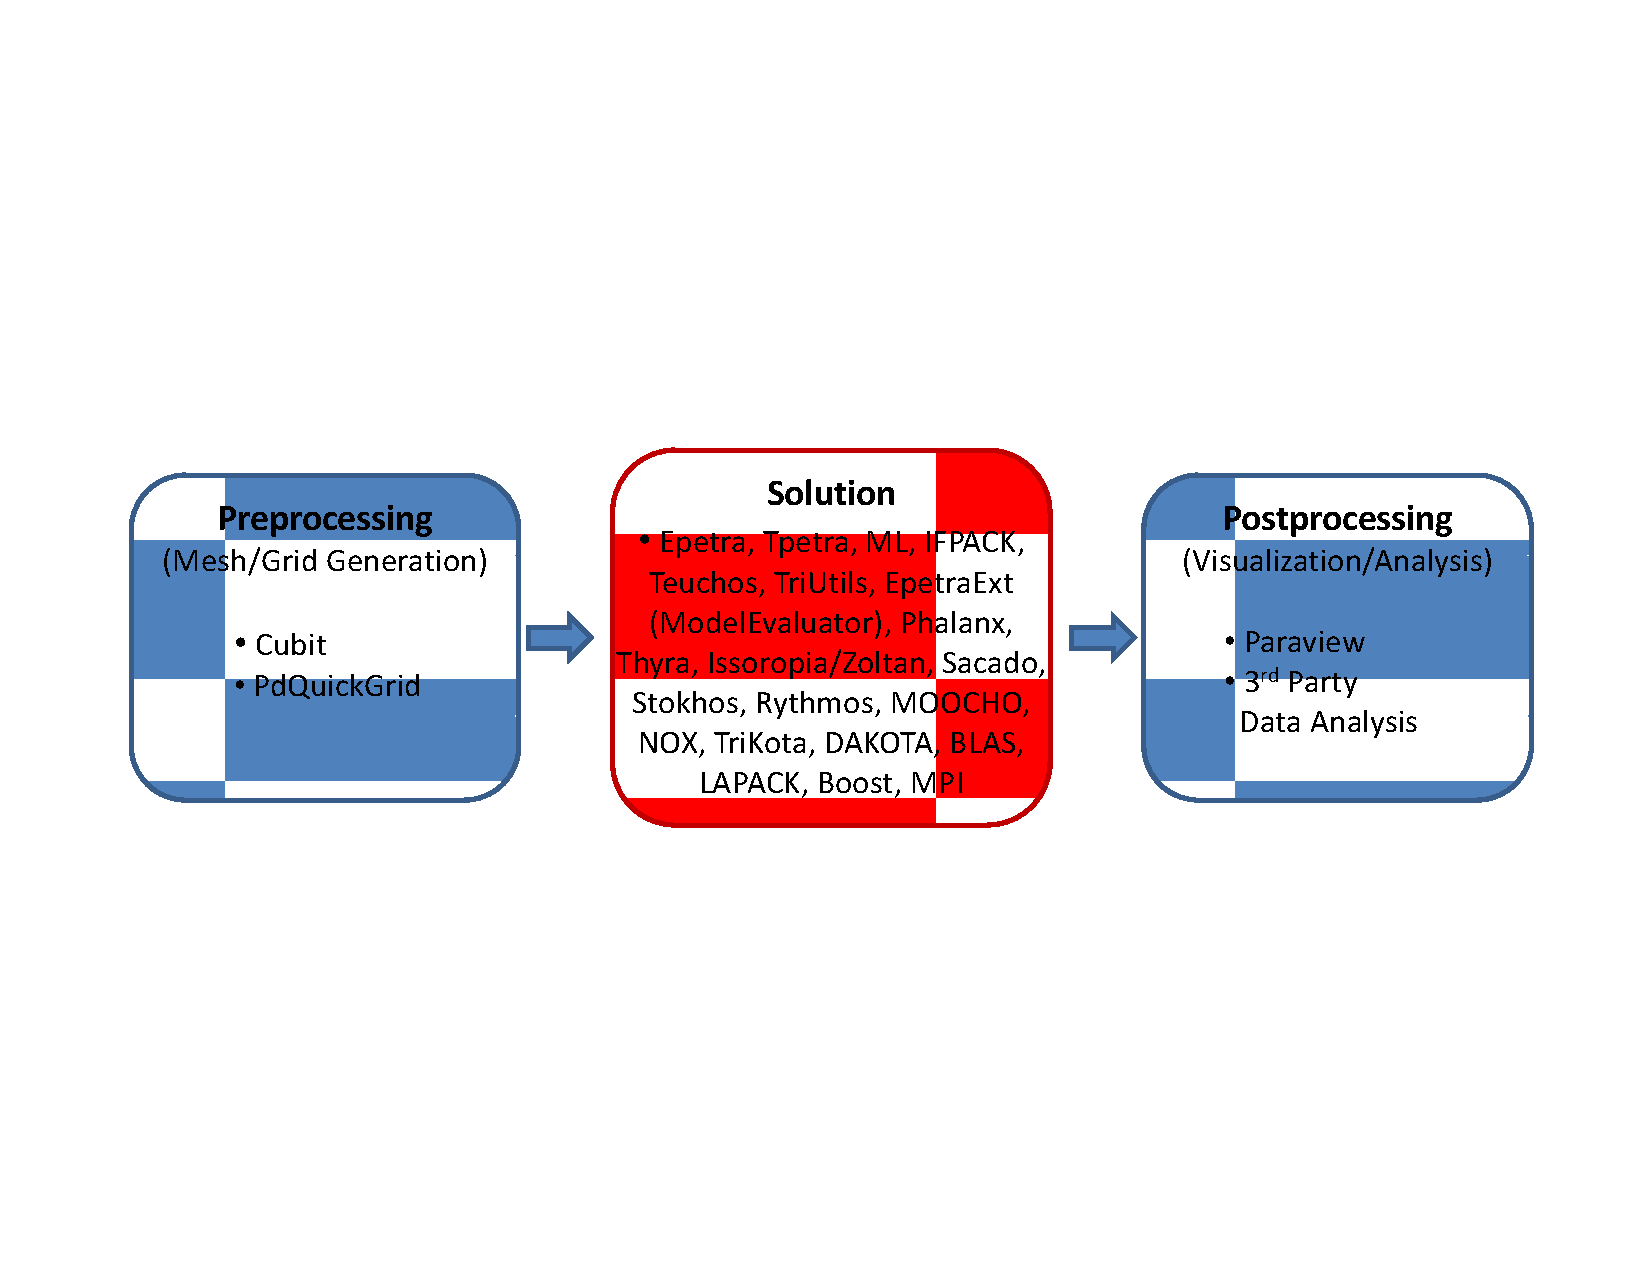
\includegraphics[scale=0.5]{PrePost}
   \end{center}
  \caption{Interaction with other software components/packages, distributed by stage of solution process.}
  \label{fig:PrePost}
\end{figure}

The software system will be constructed utilizing Trilinos components. Figure \ref{fig:TrilinosComponents} shows some of the functionality provided by Trilinos, and its expected order of integration into the software system.
\begin{figure}[h!]
  \begin{center}
   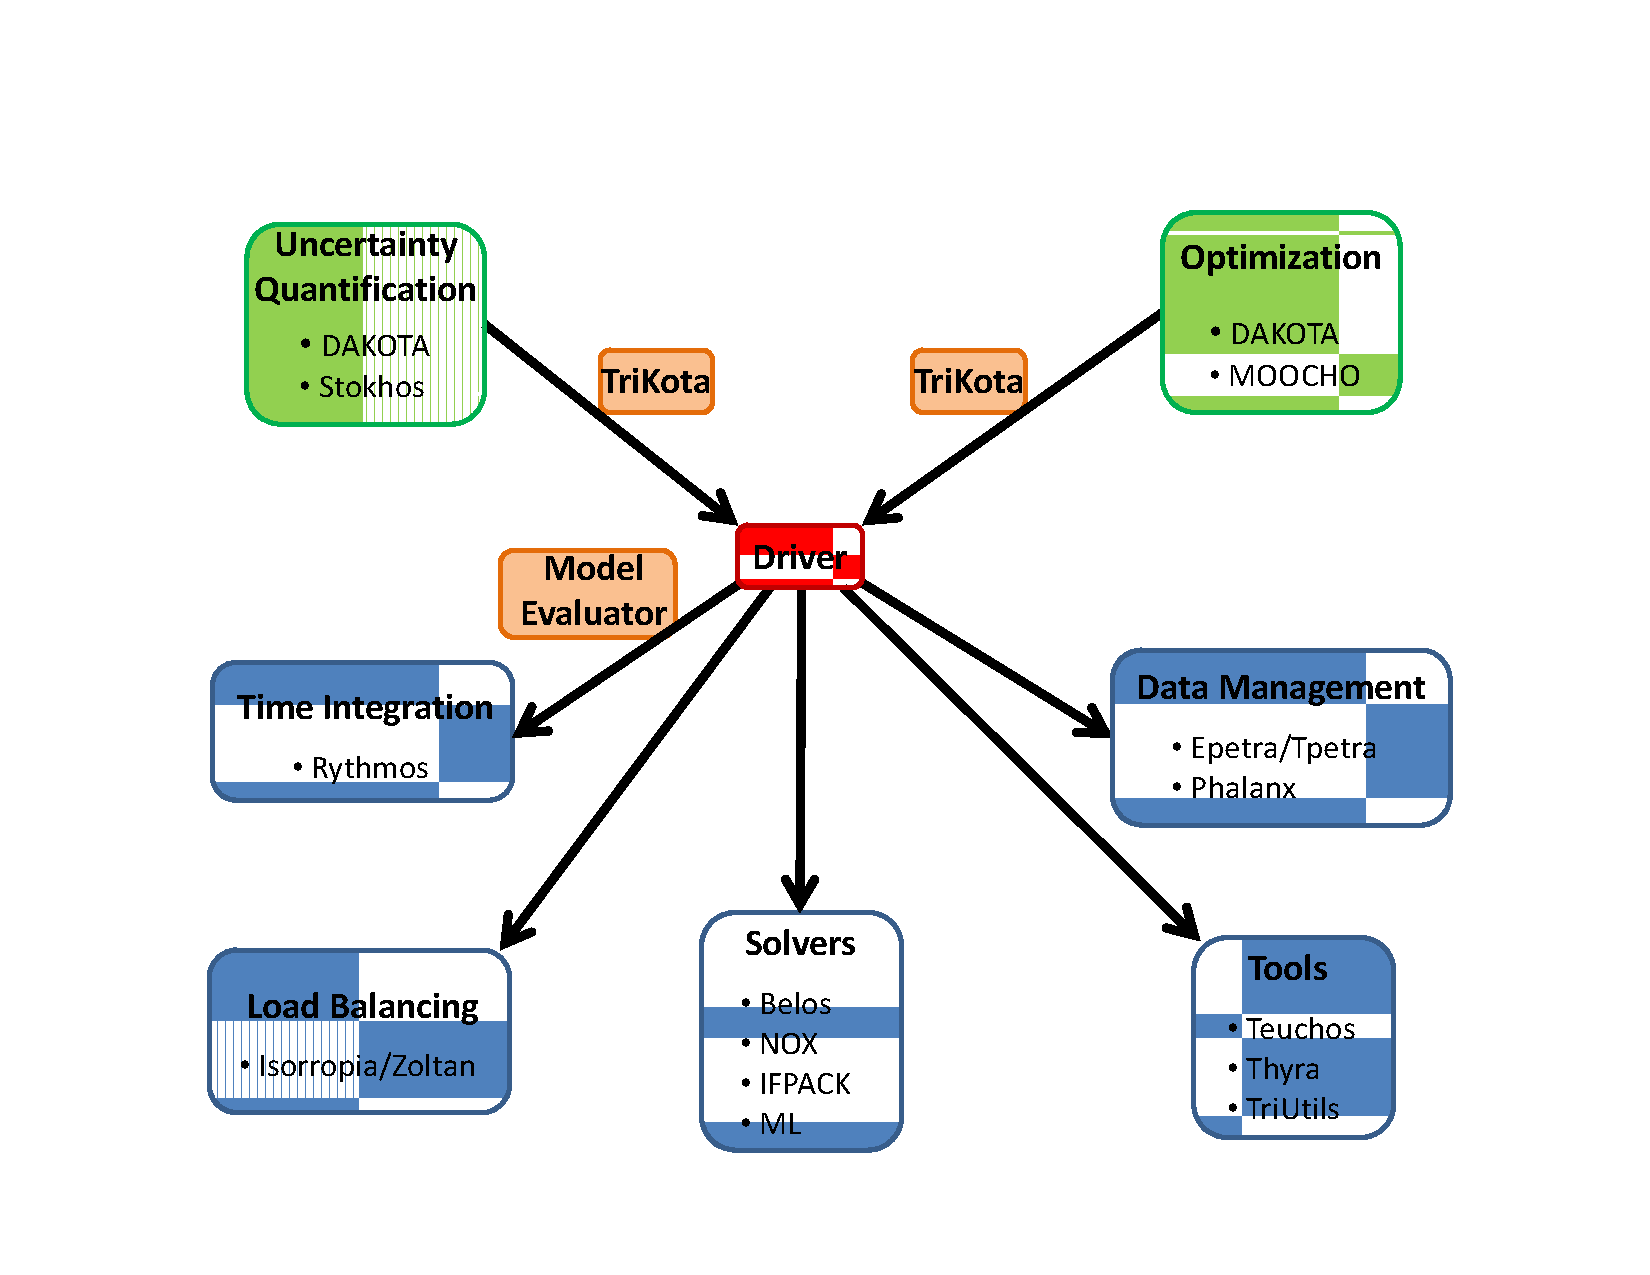
\includegraphics[scale=0.6]{TrilinosComponents}
   \end{center}
  \caption{Interaction with other software components/packages used in solution stage, distributed by functional role.}
  \label{fig:TrilinosComponents}
\end{figure}

To provide for UQ and optimization, the software system will interface with the DAKOTA project via the \emph{TriKota} Trilinos package. TriKota automates the interface between DAKOTA and Trilinos-based codes, shown in Figure \ref{fig:DakotaInterface}.
\begin{figure}[h!]
  \begin{center}
   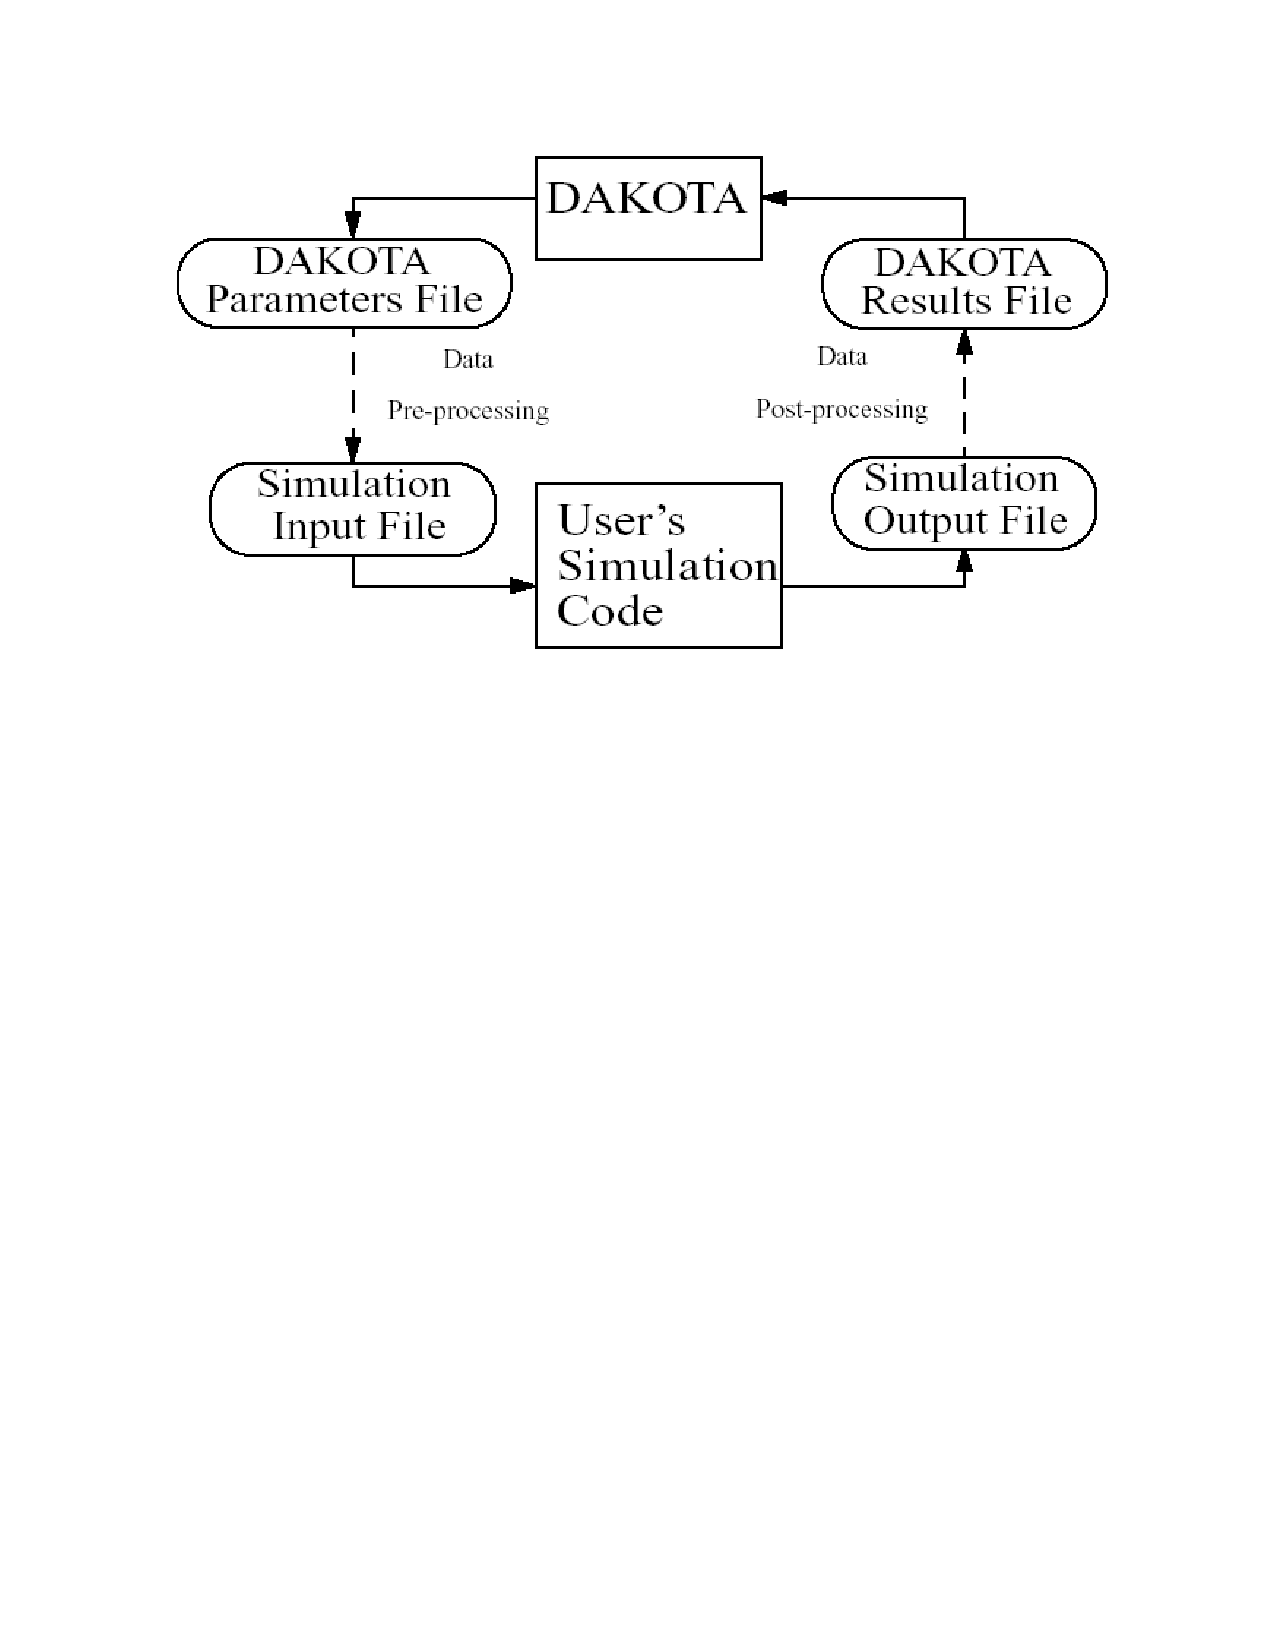
\includegraphics[scale=0.6]{Dakota}
   \end{center}
  \caption{The loosely-coupled or ``black-box'' interface between DAKOTA and a user-supplied simulation code. For Trilinos software products, this functionality is achieved with the \emph{TriKota} package. Image courtesy of \cite{Eldred:2008:Dakota}.}
  \label{fig:DakotaInterface}
\end{figure}

\subsection{Product functions}

This software system will accept an input script and (possibly) other input data files describing materials and geometry, and perform a serial or parallel single- or multi-physics simulation based upon commands given in the input script. Simulations are either \emph{dynamic} or \emph{static}. \emph{Explicit} and \emph{implicit} time integrators are provided. Data will be output to disk (and optionally to the screen) as the simulation proceeds, followed by summary information when the simulation terminates.  A more detailed description of the functions performed by this software system is given in Section~\ref{sec:Requirements}.

\subsection{User characteristics}

It is assumed that users are knowledgeable in the physics they desire to simulate, and can specify peridynamic kernels appropriate to those physics (selecting from provided kernels if appropriate). It is also assumed users understand how to couple between these physical models (selecting from provided couplings if appropriate). We assume users have the skill to implement their own kernels and multiphysics couplings using provided hooks in the software if the kernels and multiphysics coupling provided in the code are not suitable for their simulations.

It is also assumed that users have at least intermediate level knowledge of the numerical algorithms employed in this software system and the other software components with which it interfaces and utilizes. For example, users are expected not to make foolish choices with regard to selection of discretizations, solvers, etc.

\subsection{Constraints}

This software system does not provide for interactive simulations. All simulations are driven via an input script or though direct coupling with a driving application, such as DAKOTA.

The primary code will be developed in C++. Developers will adhere to good software development practices. Parallelism will be achieved through MPI or through already-parallelized Trilinos components built upon MPI.  Reliability is highly desirable -- the code will exit gracefully upon failure or error, returning an informative error message.

Developers will utilize automated daily regression testing and pre-checkin tests.  The test suite will contain, among other things, problems whose analytic solutions are known. (See ``verification tests'' in \S\ref{sec:OtherRequirements}.) Basic correctness of code will judged by the ability of the code to reproduce analytic solutions up to the error introduced by numerical methods.

\comment{
\MLP{Dave: Can you say more about acceptance tests? What's done for Sierra mechanics? Mostly comparison of numerical solution to analytic solution (for cases where analytic solution is know)? Does it make sense for us to use any tests from Sierra?}
}

\subsection{Assumptions and dependencies}

This software system depends upon the Trilinos project \cite{Heroux:2005:Trilinos} and the DAKOTA project \cite{Eldred:2008:Dakota}, and assumes the correctness, completeness, and stability of these software projects. This software system is also then dependent upon all TPLs that utilized Trilinos packages are dependent upon (for example, BLAS, LAPACK, Boost, etc.) Further, the developers assume cooperation from Trilinos and Dakota developers in implementing any functionality in their packages deemed critical to the success of this project.

It is assumed the users will generate their own geometries and meshes via other third-party packages (e.g., Cubit), although we will provide mesh-generation tools for simple regular geometric solids. It is assumed the users will utilize other third-party packages for post-processing of data, including visualization (e.g., Paraview.) We will provide the capability for the user to specify in the input script an output format format suitable for direct input to a visualization package. (For example, the user could specify in the input script that the output be written directly to the VTK or Exodus formats, which are both readable by Paraview.)

%%% ----------------------------------------------------------------------
\section{Specific Requirements} \label{sec:Requirements}

\subsection{External interface requirements}

\subsubsection{User interfaces}

The user will interface with the code through input scripts and other input files, and also through output data files generated by the software system. Documentation and syntax of input script commands will be provided on a webpage or wiki. Sample input scripts will also be provided with the source distribution. The software system will provide a checkpoint/restart capability, allowing users to restart a computation from a restart file.

\subsubsection{Hardware interfaces}

Initial support only for RedHat, MacOS, and operating systems run by massively parallel DOE machines.

\subsubsection{Software interfaces}

This software system will interface with and directly utilize many packages within Trilinos, as well as linking with DAKOTA. The VOTD of this software system will build against the last stable VOTD of Trilinos and DAKOTA.  Software that utilizes Peridigm modules, e.g.~Sierra Mechanics, is expected to maintain compatibility with the last stable VOTD of Trilinos.

Specifically, we are likely to utilize the following software packages:
\begin{description}
  \item[Epetra:] Parallel numerical linear algebra. Also provides wrappers for BLAS \& LAPACK.
  \item[Tpetra:] Next-generation, templated version of Petra.
  \item[ML:] Multilevel solvers.
  \item[Belos:] Next-generation iterative solvers.
  \item[IFPACK:] Distributed algebraic preconditioner package.
  \item[Teuchos:] Common tools package.
  \item[TriUtils:] Further Trilinos utilities.
  \item[EpetraExt:] Matrix/Vector read/write utilities. Also contains \emph{ModelEvaluator}, a nonlinear model evaluator.
  \item[Phalanx:] Local field evaluation kernel.
  \item[phdMesh:] Parallel Heterogeneous Dynamic unstructured Mesh (phdMesh) data structure library.
  \item[Intrepid:] Compatible discretization library.
  \item[Cubit:] Geometry and mesh generation toolkit.
  \item[Thyra:] Set of interfaces and supporting code that defines basic interoperability mechanisms between numerical software.
  \item[Issoropia/Zoltan] Parallel dynamic load balancing and related services.
  \item[Sacado:] Automatic differentiation package.
  \item[Stokhos:] Intrusive stochastic Galerkin uncertainty quantification methods.
  \item[Rythmos:] Time integration methods.
  \item[MOOCHO:] Multifunctional Object-Oriented arCHitecture for Optimization, a package for nonconvex optimization.
  \item[NOX:] Nonlinear solvers.
  \item[TriKota:] Trilinos/DAKOTA interface.
  \item[DAKOTA:] Algorithms for optimization with gradient and nongradient-based methods; uncertainty quantification with sampling, reliability, polynomial chaos, and epistemic methods; parameter estimation with nonlinear least squares methods; and sensitivity/variance analysis with design of experiments and parameter study methods.
  \item[BLAS:] Basic linear algebra subroutines.
  \item[LAPACK:] Dense serial linear algebra.
  \item[Boost:] Template metaprogramming library (MPL).
  \item[MPI:] Message passing library.
\end{description}

\subsubsection{Communication interfaces}

No communications interfaces are supported.

\subsection{Functional Requirements}

Peridynamic simulations will be driven via an input script.  The input script will contain information related to initialization, simulation, output, and termination.

\paragraph{Validity checks on inputs.}

Minimal validity checking will be performed. Validity checking will be limited to ensuring all necessary input is present for a simulation. (For example, ensuring the user has specified a mesh and at least one peridynamic model before beginning simulation.) Validity checking of input will occur at the time that portion of the input script is processed.

\paragraph{Initialization.}

The user shall specify
\begin{itemize}
  \item a discretization (either as a file of mesh and connectivity information to be read in) or as a discretization supported internally by Peridigm (e.g., a regular geometric solid.)
  \item a material type (from the material library)
  \item desired peridynamic physics (embodied by a specific peridynamic kernel function) as well as coupling operations between peridynamic physics
  \item a solver (e.g., explicit time integrator and supporting parameters)
  \item output to disk and/or screen (optional)
\end{itemize}

It is assumed for initial versions of code that only discretizations of the strong form of the peridynamic operator are used, essentially following the method proposed in \cite{Silling:2005:Meshfree}.

Initialization will occur following the reading of input data files and processing of the initialization section of the input script.  The initialization phase includes initializing all variables and fields, handling parallel distribution of data, and initial load balancing.

\paragraph{Simulation.}

The user shall specify a command in the input script to run the simulation. The chosen time integrator or other solver drives the simulation. Via the ModelEvaluator interface, the peridynamic simulation code returns response variables to the time integrator. The code also handles the inter-processor communcation necessary to evaluate integrals of peridynamic kernel functions. Periodic load balancing shall occur as required for efficient computation. Output generated by the simulation shall be written to disk and/or screen, as specified in the input script.

\paragraph{Termination.}

Following the analysis prescribed in the input script the software system cleans up memory and closes files, reporting summary data to screen and/or disk as specified.

\subsection{Performance Requirements}

The software system is expected to achieve reasonable serial and parallel performance.  Scaling tests will be constructed for evaluating parallel performance over a variety of problem sizes to identify possible performance bottlenecks.

\subsection{Design constraints}

The ModelEvaluator framework (EpetraExt) and/or associated Thyra wrappers are required for directly compatibility with a number of Trilinos packages.  Interfaces in the software system must be designed accordingly.

\subsection{Software system attributes}

\paragraph{Reliability.} The software system shall pass all unit and regression tests. ``Almost continuous integration'' will be utilized, keeping code current with Trilinos and DAKOTA VOTDs.

\paragraph{Availability.} The software system shall support checkpointing, recovery, and restart functionality.

\paragraph{Security.} None.

\paragraph{Maintainability.} The software system shall be highly modular, as it is built upon Trilinos components, and utilize accepted means of connecting together those components. The software system shall modularize peridynamic kernel functions, allowing them to be easily added or modified. In particular, interfaces will be provided to both peridynamic constitutive models and classical material models, discussed below.
\begin{description}
  \item[Peridynamic Constitutive Models:] These material models, such as the linear peridynamic solid (LPS) model, will reside in the \verb"src/materials" directory, and will all inherit from a common base class, thus presenting the same interface to the Peridigm code. This interface will facilitate the direct passing of deformation state data to the material model and the direct processing of subsequent force evaluations computed within the material model. Further, this interface allows end users to easily add their own peridynamic materials to the material library.
  \item[Classical Constitutive Models:] For these material models (e.g., those used in classical finite element codes), a special material model interface will be provided, as discussed in \cite{Silling:2007:PDStates}. The classical material model interface will allow for the passing of the peridynamic approximation of the deformation gradient (or quantities derived therefrom) to the material model. Additionally, the classical material model interface will contain functionality for converting stresses computed by a classical material model into force state data applicable to peridynamics.
\end{description}
To ensure compatibility with various Trilinos components (e.g., \verb"EpetraExt::ModelEvaluator"), the Peridigm material interfaces will require material models to be stateless, i.e. no data will be stored within a material model.  To accommodate history-dependent material models, Peridigm will allow for the storage of history-dependent material state data in a way that is both external to the material model itself and compatible with the Rythmos and NOX solvers provided in Trilinos.

\paragraph{Portability.} The software system will be developed initially for a limited range of platforms, but will utilize as much platform independent code as possible. The build system shall be CMAKE, a platform-independent build system.

\subsection{Other requirements} \label{sec:OtherRequirements}

This section is devoted to a discussion of developer tools and resources that will be utilized.

\paragraph{Project Management Software}

We will utilize \emph{Trac}, an open source project management tool. Trac is a lightweight project management tool that is implemented as a web-based application, written in the Python programming language. It emphasizes ease of use and low ceremony, and is open source. Trac supports many features, including a ticket system, progress tracker, online repository browsing and management, user management, a wiki, and other features available through plugins. the trac site is located at \url{https://development.sandia.gov/trac/peridigm}.

\paragraph{Compilers}
The primary compilers utilized will be the gcc (GNU compiler collection) v.4.x.x.  Additionally, supporting shell or python scripts will be used.

\paragraph{Build system.}
Configuration and building will be managed with CMAKE.

\paragraph{Version Control.}
Subversion will be used to manage the software system.

\paragraph{Issue Tracking}
Trac will be used for issue/ticket/bug tracking. This may require customized third-party plugins for Trac, including but not limited to TracIncludeMacro, TracNav, TracDownloader, TracSpamFilter, and the TracTicketModerator plugin (developed by Sandia) for moderated ticket submission.

\paragraph{Software Testing}
Multiple test suites will be developed and maintained for the software:  unit tests, regression tests, performance tests, and verification tests.  The software and test suites will be monitored for memory errors using appropriate utilities (e.g.~valgrind, libgmalloc), and test coverage will be monitored using a suitable coverage tool (e.g. gcov).

\subparagraph{Unit Tests.}
Unit tests will be constructed using the Boost unit-testing framework.

\subparagraph{Regression Tests.}
A regression test suite will be developed and maintained to reduce the introduction of bugs as new code is added to the software system.  The CTest utility will be used to manage the regression test suite.

\subparagraph{Performance Tests.}
A performance test suite will be developed and maintained to monitor code performance and scalability when performing large-scale analyses.  The CTest utility will be used to manage the performance test suite.

\subparagraph{Verification Tests.}
A verification test suite will be developed and maintained to demonstrate the software's ability to correctly simulate material response in a set of problems with known solutions. The CTest utility will be used to manage the verification test suite.

Each verification test will include a short write-up describing the test, along with computational and theoretical results. The collection of verification tests will comprise a verification manual for Peridigm. Theoretical solutions to peridynamic integral equations can be derived following results in \cite{Weckner:2003:PDBar1,Weckner:2005:PDBar2,Weckner:2009:PDGreens}.

\paragraph{Wiki and Web Resources}
We will utilize the Trac wiki to provides access to software documentation, release history, and access to the Peridigm subversion repository.

\paragraph{Mailing List(s)}
We will utilize mailing lists (via \emph{MailMan}) on development.sandia.gov.

\appendix
\section{Feature Implementation Outline}

\subsection{Initial Implementation}

Simple driver application to solve a state-based PD linear elastic solid mechanics problem with no short-range forces (essentially, a simplified exploding cylinder problem.) The solution will be driven by a Rythmos time integrator (explicit time integration only) using velocity initial conditions.  The software will be constructed using Epetra parallel data structures/functionality and the ModelEvaluator interface.

Specific functionality includes the ability to:
\begin{itemize}
  \item Generate mesh for cylinder problem [Status: In progress.]
  \item Distribute mesh/bond data into Epetra data structures [Status: Completed.]
  \item Return force state for state-based linear peridynamic solid material model [Status: Completed.]
  \item Call time integrator (Rythmos) [Status: Completed.]
  \item Write output to file [Status: In progress.]
\end{itemize}

\subsection{Future Implementation}

By quarter for FY10, the remaining milestones are:

\begin{description}
  \item[Q2] Implement core functionality for single-physics simulation. This is complete when we can explode a (mechanical)cylinder (with bond breaking) in parallel. (No short range forces.)
  \item[Q3] Implement core functionality for multi-physics simulation. This is complete when we can explode a (thermo-plastic) cylinder (with bond breaking) in parallel. (No short range forces.)
  \item[Q4] Multi-physics demonstration problem: cylinder fragmentation. This is complete when we can explode a thermo-plastic cylinder (with bond breaking and short-range forces) in parallel, and connect to Dakota for optimization/UQ.
\end{description}

More specific implementation tasks are listed below. Not all of these are necessary for the FY10 year-end deliverable, but all are desirable features.
\begin{itemize}
  \item Implement multiple physics models and methods coupling between different physics via Phalanx. Specifically, heat transfer and solid mechanics.
  \item Utilize Zoltan for periodic load balancing and parallel data movement.
  \item Implement short-range force calculations, including efficient construction and updating of a neighbor list.
  \item Allow for applied boundary conditions.
  \item Connect to DAKOTA for optimization and UQ.  Target problem is the analysis and optimization of the fragment size distribution of an exploding cylinder.
  \item Implement additional material models, e.g.~elastic-plastic PD solid.  Create interface for linking with classical mechanics material models.
  \item Read mesh data file (including neighborlist information) from disk.
  \item Implement checkpoint/restart functionality for use with large-scale analyses.
\end{itemize}

\end{document}
